\section{Selection}
\label{sec:hhh:sel}

Signal candidates for the decays \btokpipimumu and \btophikmumu must first pass the \lone muon
trigger.
Subsequent software trigger stages required that at least one final-state muon has $\pt>1.0\gev$
and at least one hadron has $\pt>1.6\gev$, both of which have an IP larger than $100\mum$ with
respect to any \PV in the event.
The response of the topological \BBDT, which was described in \Sec{sec:lhcb:trig}, in \hlttwo must
be consistent with a decaying $B$ meson with muons in the final state.

%There is large overlap between the...

Candidate \Bp hadrons are then formed from combinations of three hadrons and a pair of opposite
sign muons.
Fully reconstructed candidates must form a good quality vertex, with a \chisq of the vertex fit
$<6$.
This secondary vertex must be well displaced from any \PV, having a flight distance inconsistent
with zero, $\chisqfd>121$.
%The angle between the \Bp candidate momentum vector and the direction defined by the PV to \Bp decay
%vertex must be less than $14\mrad$.
Each track must satisfy $\chisqip>16$, where the \chisqip of a track is defined as the change in
\chisqip when calculated with and without the track in question.
The muons must both satisfy the \ismuon criteria and have $\dllmupi>0$,
while \pid criteria for hadrons are applied later.
Each hadron must have $\pt>500\mev$ and
the total invariant mass of the \kpipi system is required to be in the range
$750<\mass{\kpipi}<2400\mev$ in order to reduced the rate of accepted events at stripping level.
For the \phik system, in additional constraint is that the \decay{\phi}{\kk} object must have an
invariant mass within $12\mev$ of $m_\phi^\pdg$.

There are other decay channels which are used throughout this analysis, specifically:
\btojpsikpipi, \btopsitwosk, and \btojpsiphik.
In all these decays \psitwostojpsipipi and \jpsitomumu.
These are each selected by requiring that both \jpsi and \psitwos candidates have an invariant
mass within $50\mev$ of their known masses~\cite{PDG2012}.

\begin{table}
  \caption{
    Selection criteria applied in the stripping.
    %The variable {\tt ADOCACHI2CUT} is the \chisq distance of the closest approach
    %(below a threshold) for all two particle combinations.
  }
  \label{tab:hhh:strip}
  \begin{center}
    \begin{tabularcuts}
      \Bp
      & \chisqvtx               &  $<$ & $6.0$ \\
      & \chisqip               &  $<$ & $16.0$ \\
      & \chisqfd               &  $>$ & $121.0$ \\\littlerule
      \kpipi
      & Vtx $\chi^2$  &  $<$ & $12.0$ \\
      %& $\mathtt{\,DIRA}$    &  $>$ & $-0.9$ \\
      & \mass{\kpipi}          &  $\in$ & $[750, 2400]$ & MeV\\
      %& ADOCACHI2CUT & $<$ & $ 20$ \\
      & \chisqip          &  $<$ & $4.0$ \\
      & \chisqfd            &  $>$ & $25.0$ \\\littlerule
      \mumu
      & \chisqvtx     &  $<$ & $12.0$ \\
      & \chisqfd                &  $>$ & $81.0$ \\
      tracks  & \chisqip     &  $>$ & $16.0$ \\
      & track $\chisq/\ndf$         &   $<$ & $2.5$ \\\littlerule
      \Kp, \pip
      & $p_T$                  &   $>$ & $500$ & MeV \\
      \mup & \ismuon  \\
      \bottomrule
    \end{tabularcuts}
  \end{center}
\end{table}




\subsection{Background contributions}
%Processes with the same final state as \btokpipimumu and \btophikmumu are not smoothly distributed
%in \mass{\kpipimumu}, rather they peak under the signal.
The tree level decays \decay{\Bp}{\jpsi\kpipi} and \decay{\Bp}{\jpsi\phik}, where
\decay{\jpsi}{\mumu}, have large branching fractions:
\begin{align}
  \BF\big(\decay{\Bp}{\jpsi\kpipi}\big)
  \cdot \BF\big(\jpsitomumu\big)
  &= (4.8 \pm 0.8)\e{-5} \\
  \BF\big(\decay{\Bp}{\jpsi\phik}\big)
  \cdot \BF\big(\jpsitomumu\big)
  &= \big(3.1 \pm 1.1\big)\e{-6},
\end{align}
and the same final state particles as the signal modes.
They therefore constitute peaking backgrounds that lie under the signal peak.
The same is true for the large contributions from \decay{\Bp}{\psitwos\kpipi} and
\decay{\Bp}{\psitwos\phik} decays, where \decay{\psitwos}{\mumu}.
These charmonium decays are large irreducible backgrounds that must be
removed with vetoes around the \jpsi and \psitwos masses.
The vetoes used remove events where the invariant dimuon mass falls in either region
$2946<m_{\mumu}<3176\mev$ or $3586<m_{\mumu}<3766\mev$.

Figure~\ref{fig:hhh:charmvetoes} shows the boundaries defined by these vetoes on data.
Mis-reconstructed decays to charmonium contribute to the upper mass sideband.
To remove these, the veto windows are extended up by $40\mev$ in the region
$5330<\mass{\kpipimumu}<5450\mev$.
Radiative tails from the decays \decay{\jpsi}{\mumu\gamma} and \decay{\psitwos}{\mumu\gamma} are
suppressed by extending the vetoes down by $250\mev$ and $100\mev$ respectively in the region
$\mass{\kpipimumu}<5230\mev$.

%However, the amount of contamination from decaying \jpsi and \psitwos is so great that both show
%evidence of asymmetric tails from

\begin{figure}
  \begin{center}
    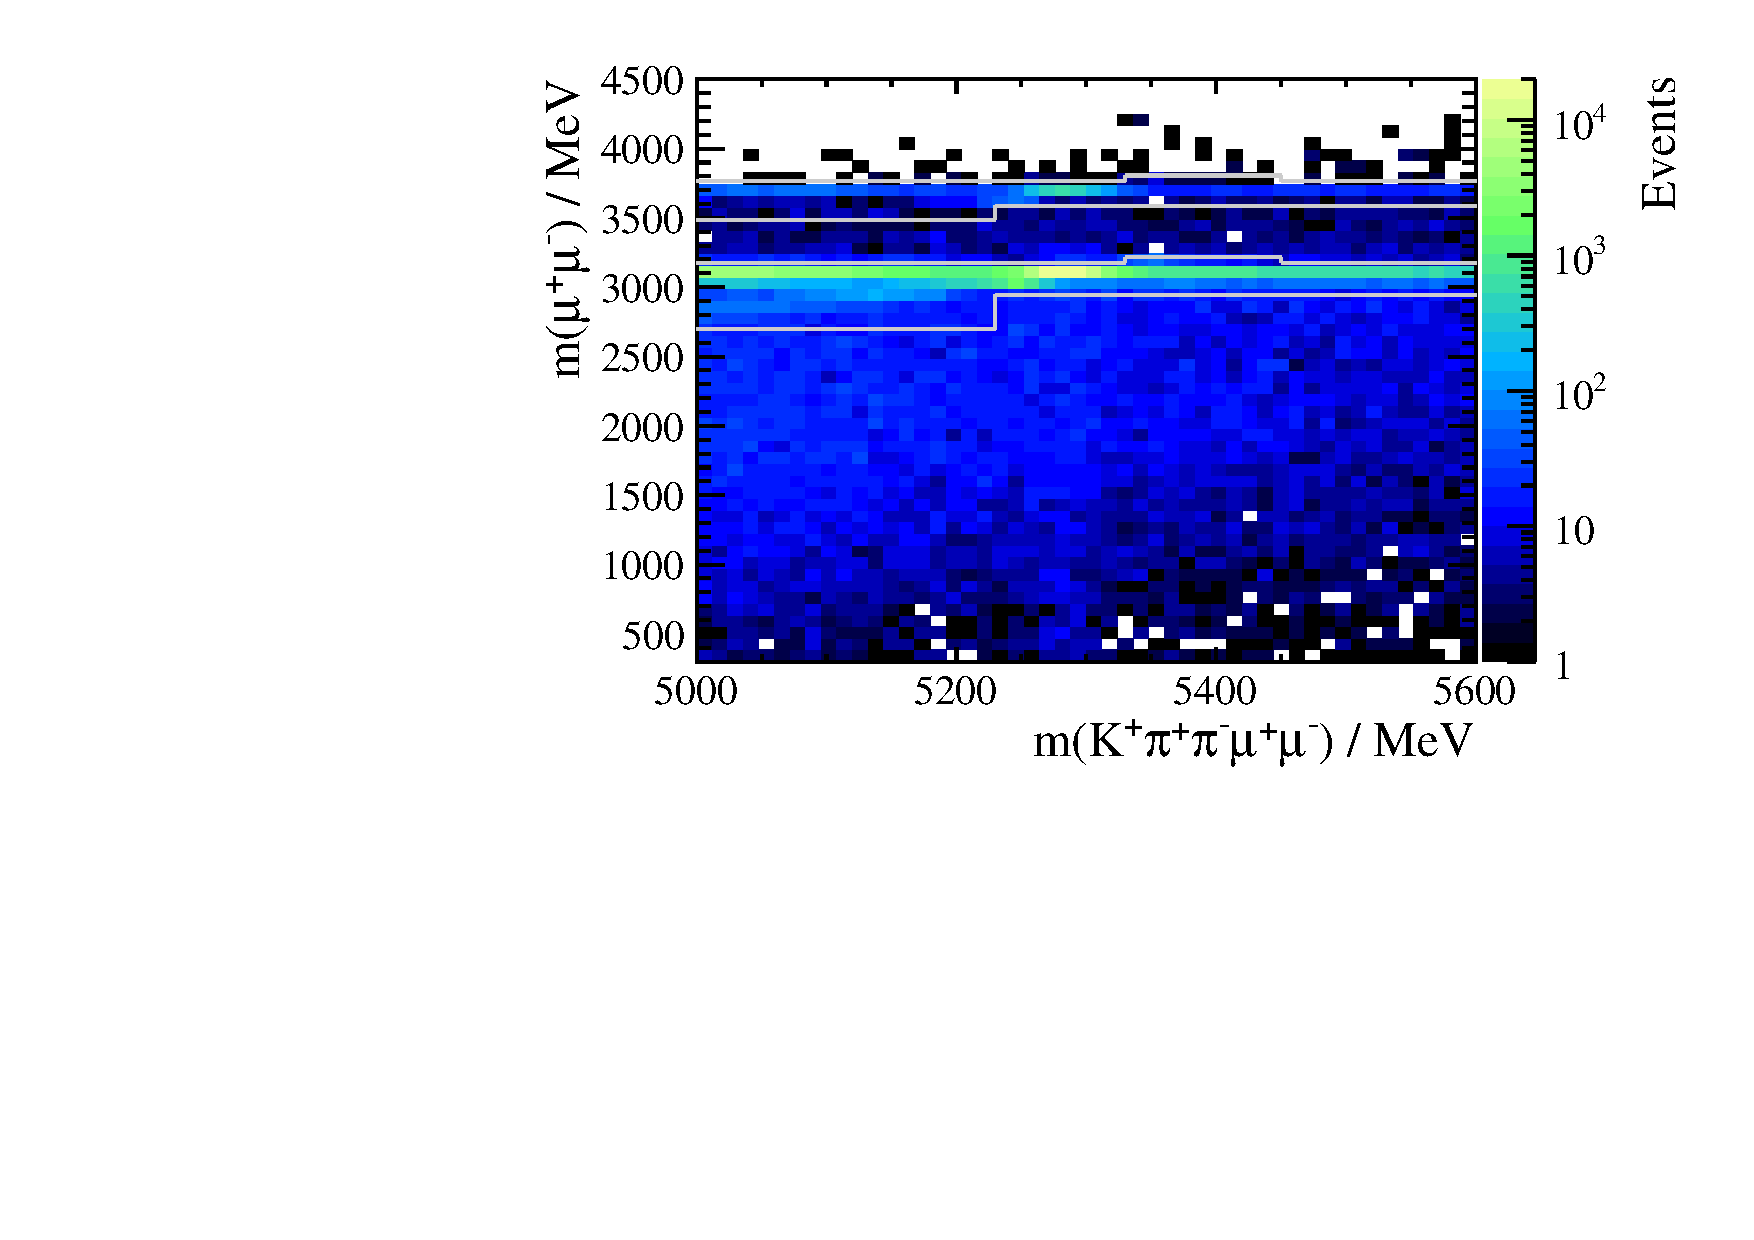
\includegraphics[width=0.48\textwidth]{BvJpre}
    %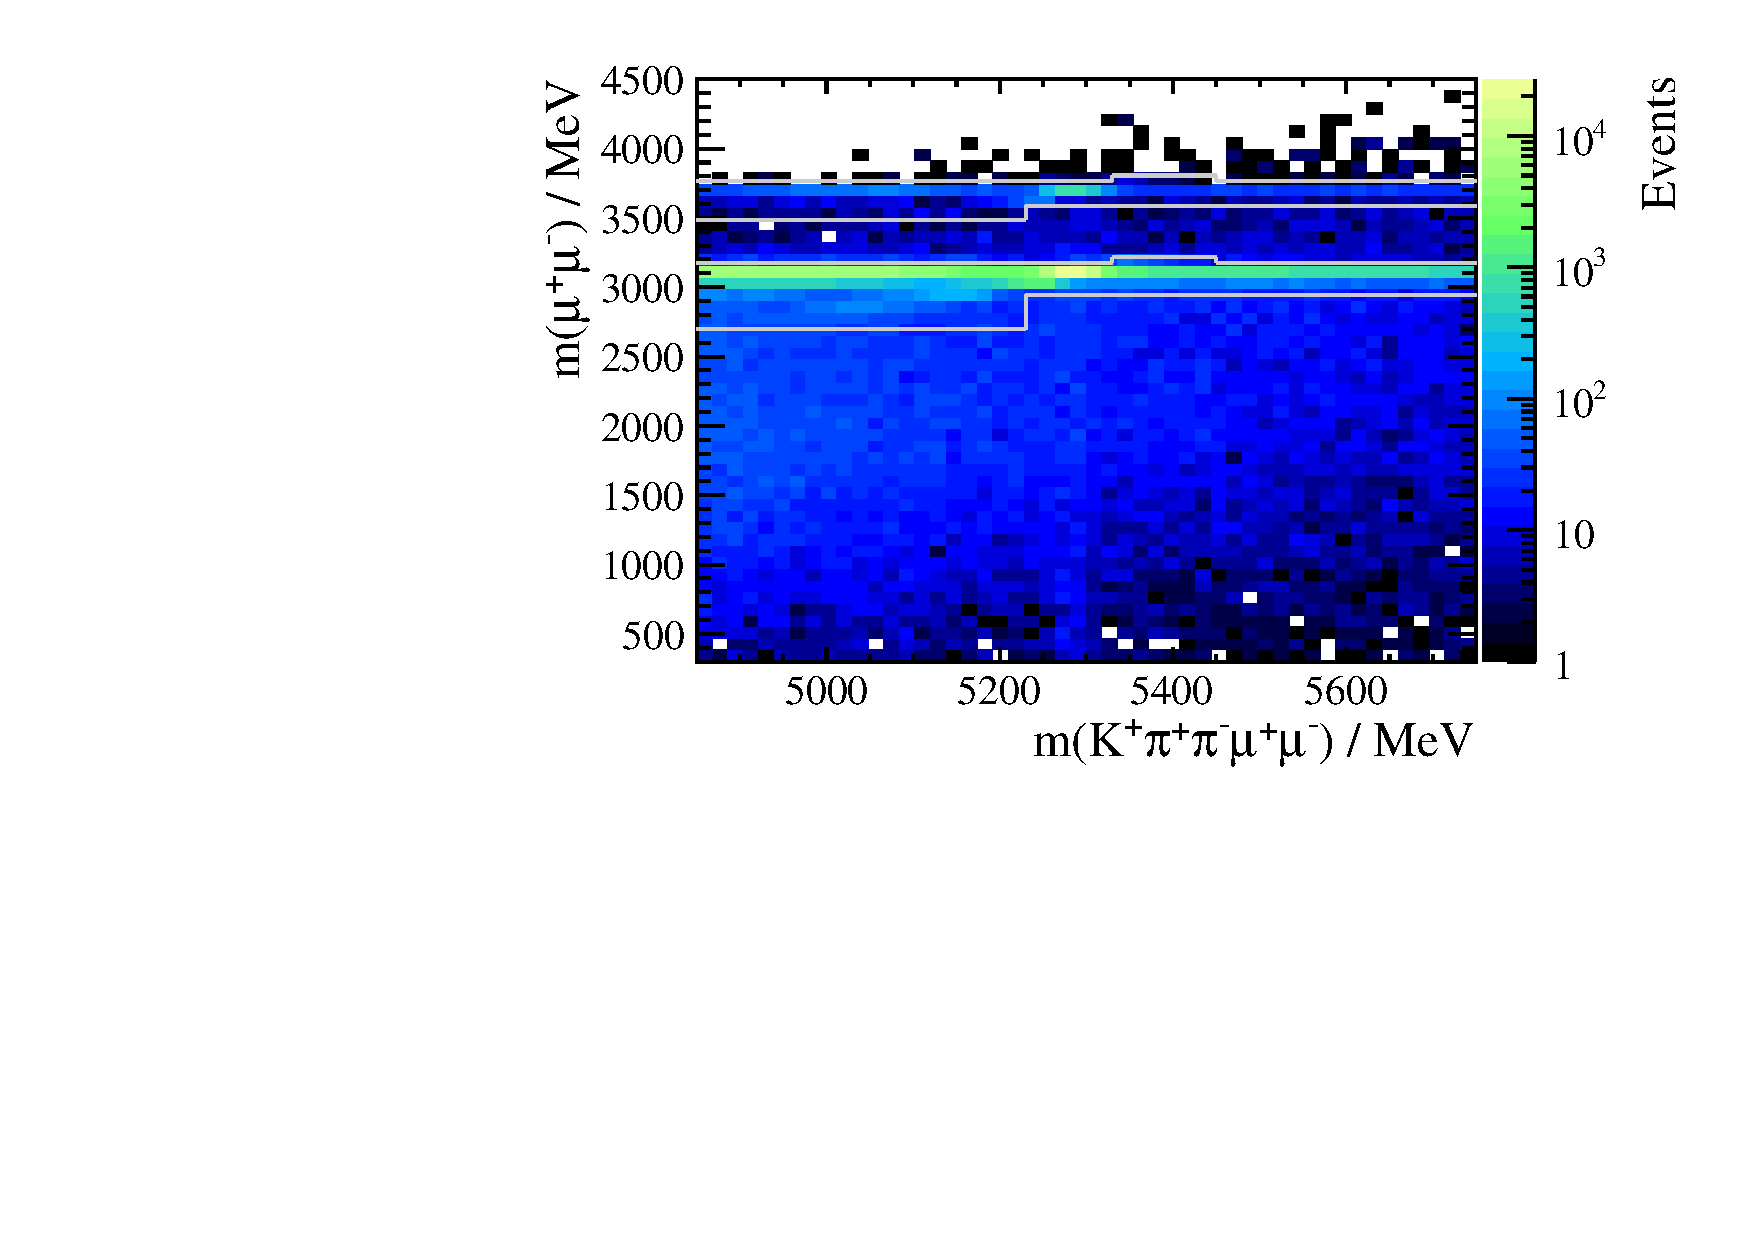
\includegraphics[width=0.48\textwidth]{BvJpost}\\
    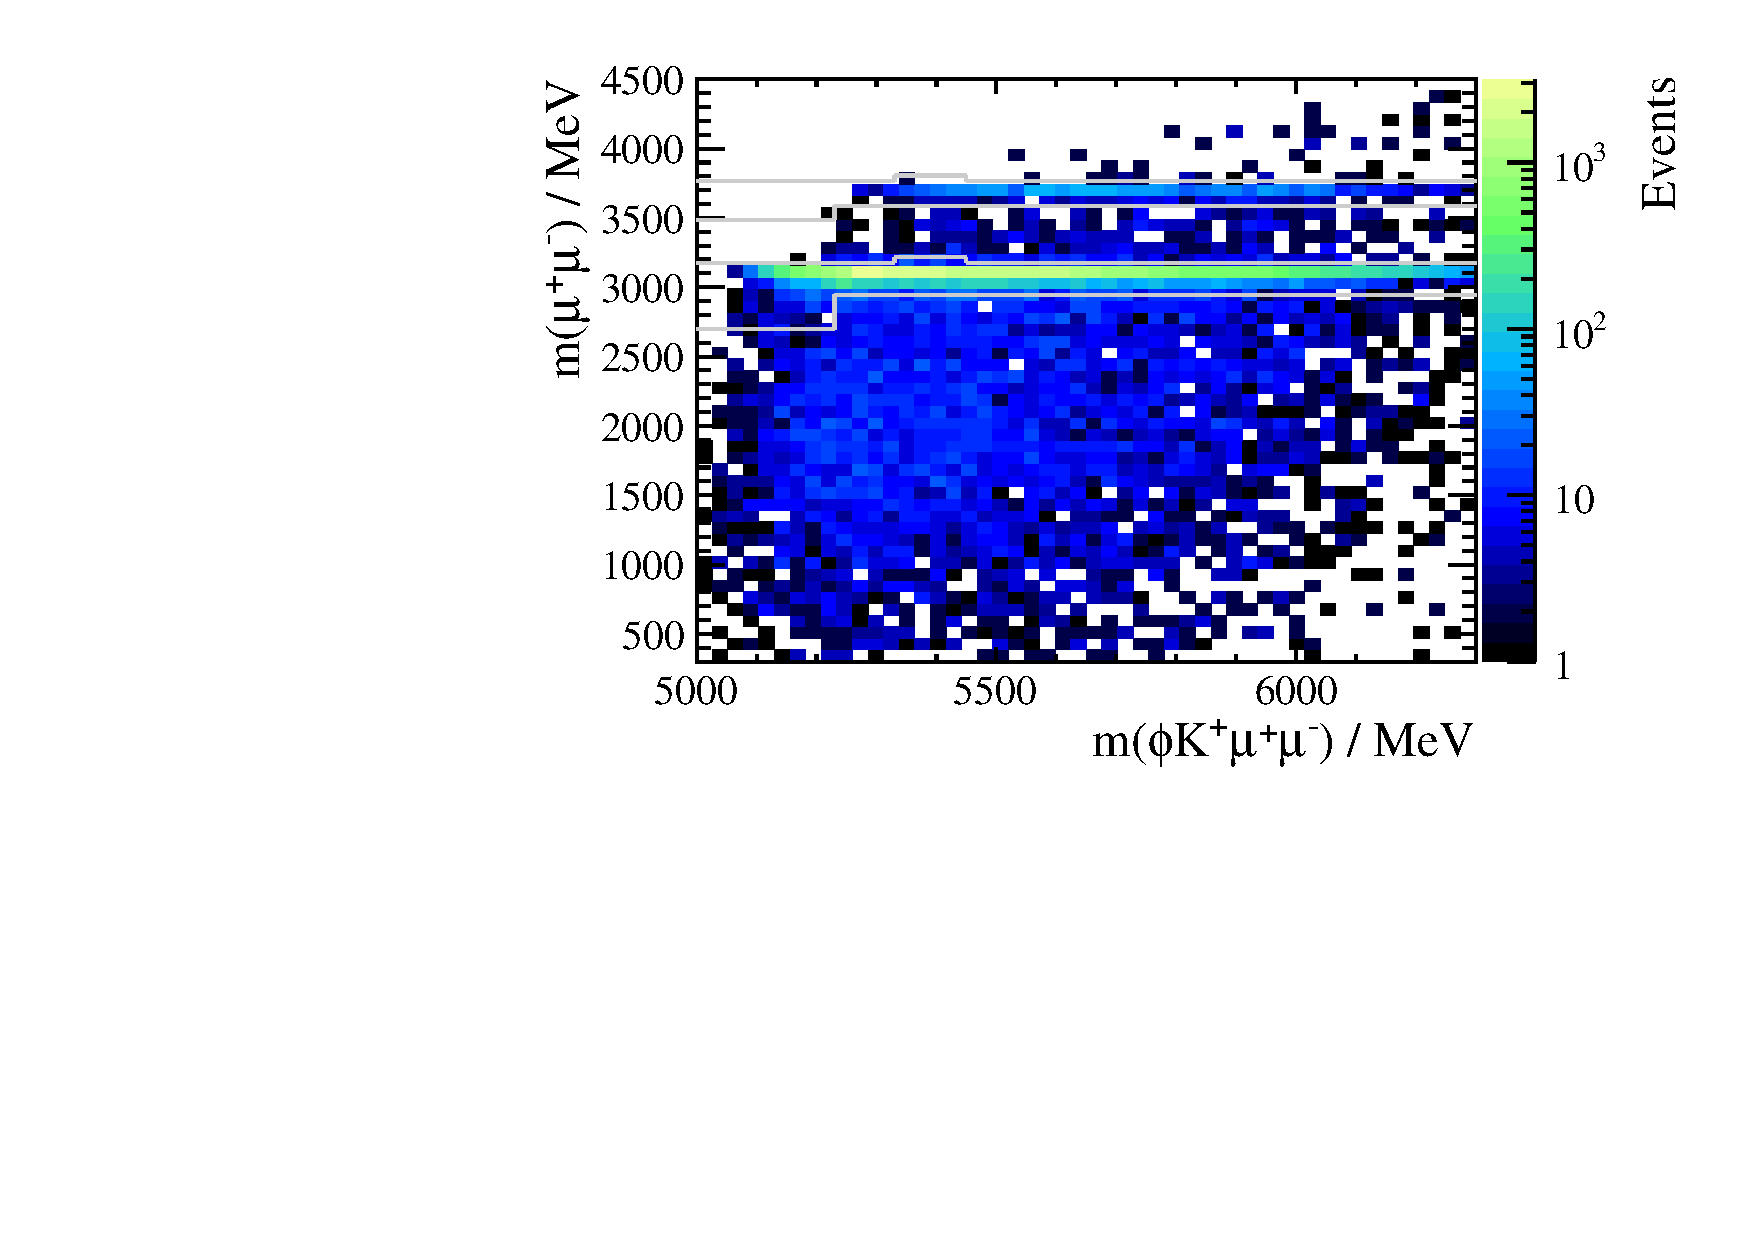
\includegraphics[width=0.48\textwidth]{BvJkkkpre}
    %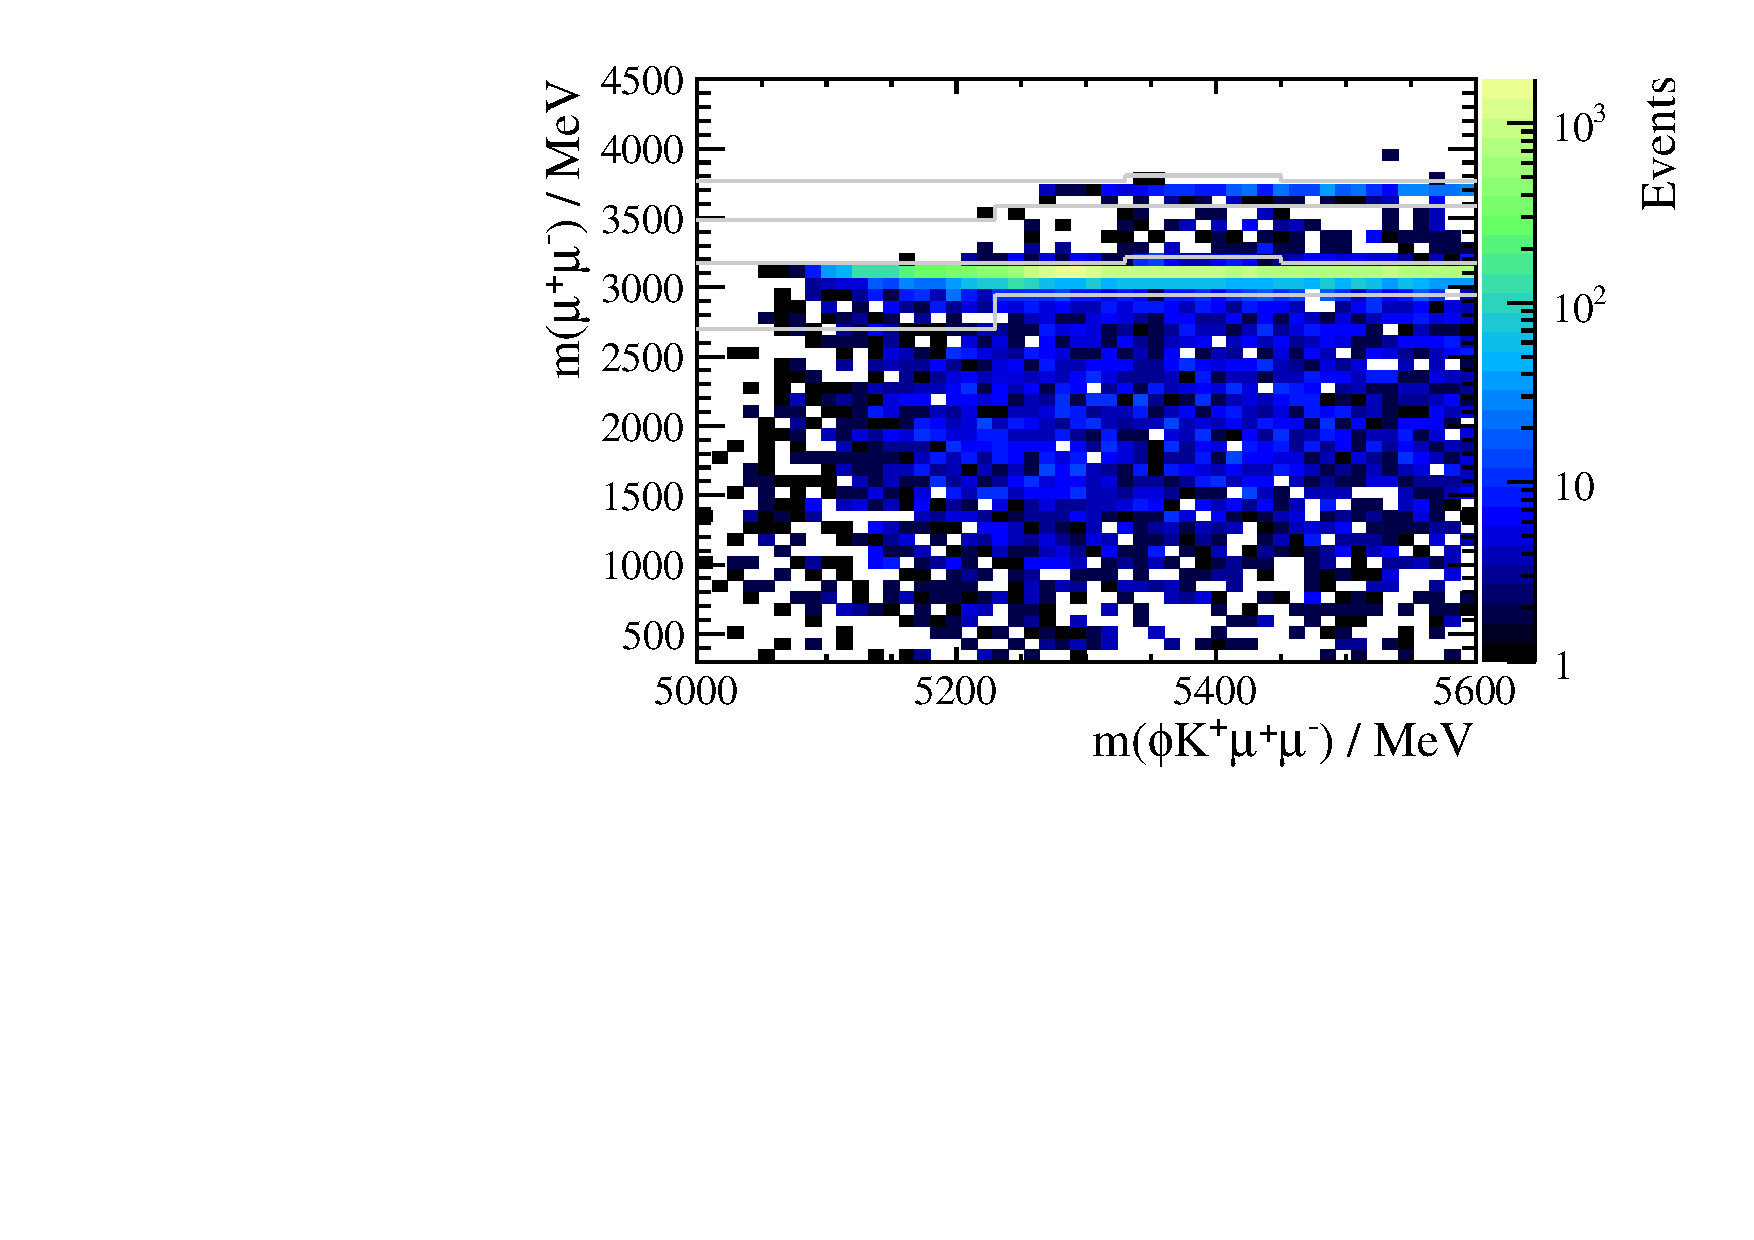
\includegraphics[width=0.48\textwidth]{BvJkkkpost}
    \caption[Charmonium vetoes is in \btokpipimumu and \btophikmumu]
    {
      The variation of the invariant mass of the dimuon candidate with the mass of the \Bp
      candidate for
      (left) \btokpipimumu, and
      (right) \btophikmumu.
      The grey lines indicate the boundaries of the charmonium vetoes.
    }
    \label{fig:hhh:charmvetoes}
  \end{center}
\end{figure}

Considering the large branching fractions of the charmonium decays given above, and the probability of
misidentifying a pion as a muon is $\mathcal{O}(1\pc)$~\cite{LHCb-DP-2013-001} (somewhat less for a
kaon) there could be significant contamination from mis-identified candidates.
This background was removed by calculating the invariant mass of each $\mu^+\pi^-$ and
$\mu^+K^-$ combination, where the hadron was assigned the muon mass.
If the mass of this object fell within $50\mev$ of $m_{\jpsi}$ or $m_{\psitwos}$, then the candidate
was vetoed.
Figure~\ref{fig:hhh:misid} shows the effect on these vetoes, and demonstrates that a large part
of the background that is removed by these vetoes is from the decay
$\decay{\Bp}{\jpsi\rho(770)^0\Kp}$.


\begin{figure}
  \begin{center}
    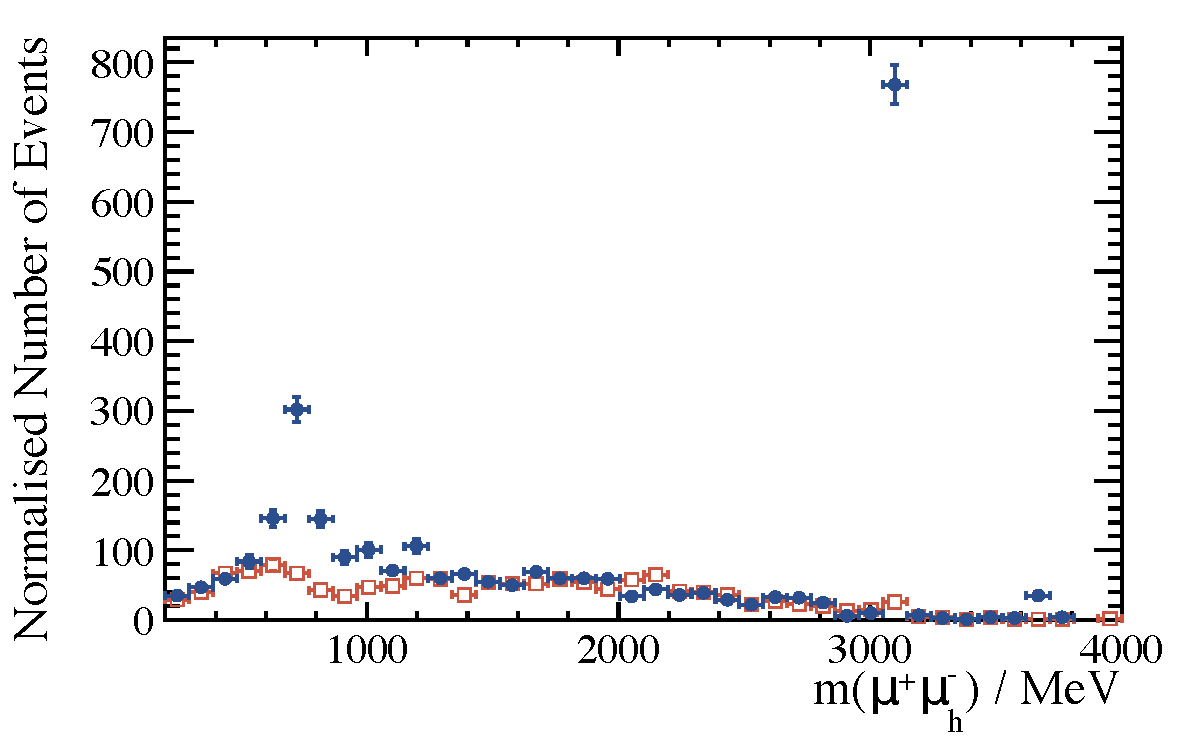
\includegraphics[width=0.45\textwidth]{hhhmisid_pre}
    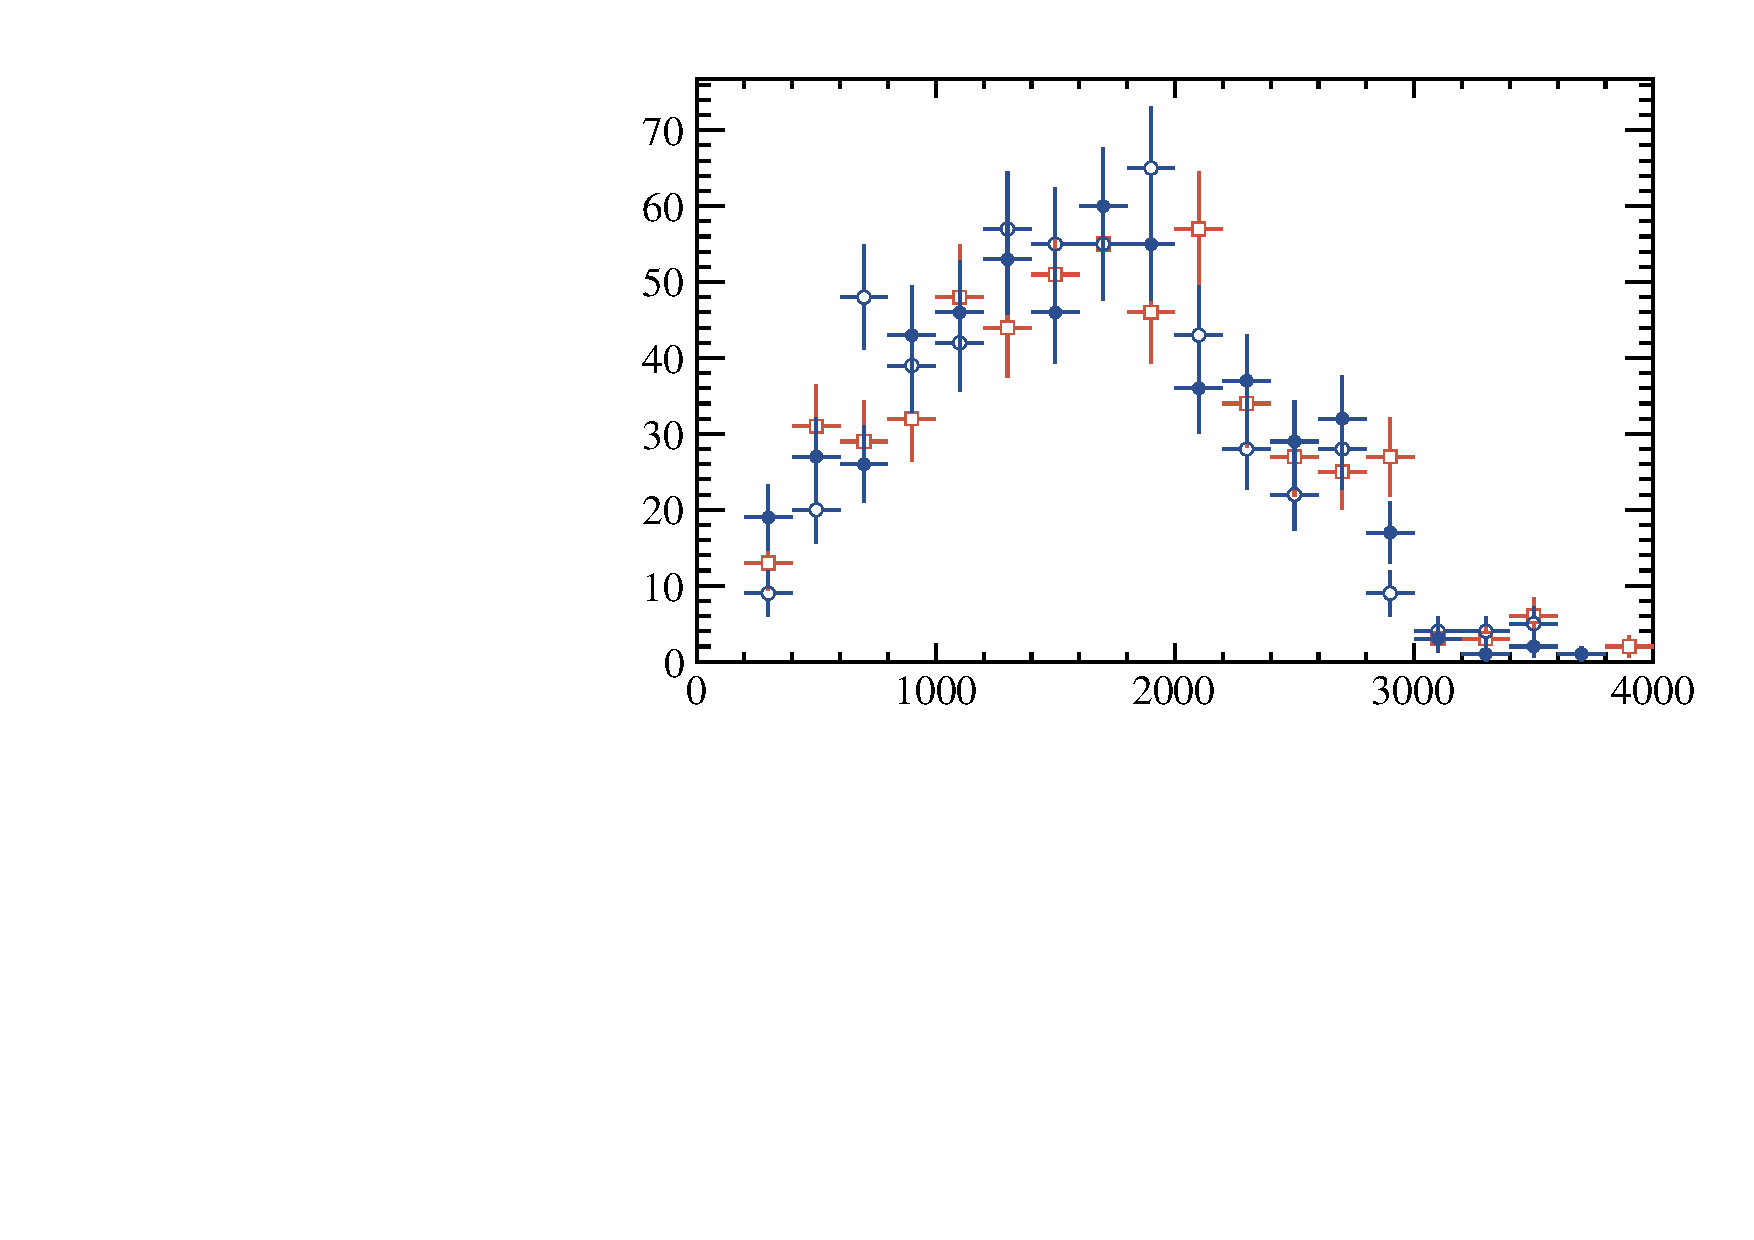
\includegraphics[width=0.45\textwidth]{hhhmisid_post}
    \caption[Backgrounds from misidentified charmonia]
    {
      Invariant mass of the combination of a muon and a reconstructed hadron of the opposite charge
      under the muon mass hypothesis (left) before, and (right) after the veto in the decay
      \btokpipimumu.
      Both pions are included in the same histogram and scaled such that it has the same number of
      entries as for the kaon.
      %The left-hand plot shows the distributions before the veto of misidentification of the \jpsi
      %and \psitwos, while the right-hand plot shows the distribution after the vetoes.
      %The blue circles are the distribution of $m(\mu\mu\to\mu\pi)$ (solid circles having the same
      %charge as the kaon) and red square show the $m(\mu\mu\to\mu K)$ distribution.
      There is a feature at low mass in the $m(\mup\misid{\mu}{\pi}^-)$ spectrum which is removed by the
      vetoes, and originates from the background decay $\decay{\Bp}{\jpsi\rho(770)^0\Kp}$.
    }
    \label{fig:hhh:misid}
  \end{center}
\end{figure}


%Other peaking backgrounds D0...
Other background contributions can come from doubly misidentified fully hadronic decays, such as
the decay \decay{\Bd}{\Dzb\pip\pipi} followed by \decay{\Dzb}{\kpi}, which
has a total branching fraction of $(2.21\pm0.85)\e{-4}$~\cite{PDG2012}.
This decay has a final state of $\kpipi\pipi$.
If a pair of opposite sign pions are misidentified
as muons, the final state of \kpipimumu is mimicked, and therefore should be considered as a
background.
The same can be said for the decay \decay{\Bd}{\Dzb\pip} and \decay{\Dzb}{\Km\pip\pipi},
which has a total branching fraction of $(3.88\pm0.15)\e{-4}$.

In order to ascertain if these charmed decays are potential backgrounds, invariant mass
distributions are inspected for evidence of \Dz mesons.
The only distribution in which there is evidence of contamination is in the
$\Kp\pi^+_\mu$ distribution\footnote{
  Where, as defined previously, the notation $h_i$ is a particle under the mass hypothesis of $h$
  which was reconstructed as an $i$.
}.
%This is shown in \Fig{fig:hhh:dzbkg}.
To remove the small possible contribution from \decay{\Bd}{\Dzb\pip\pipi} events which fall within
$30\mev$ of the nominal \Dz mass in the $\Kp\pi^-_\mu$ spectrum are vetoed.
%\bam{PLOT.}


% SEMILEPTONIC DECAYS
Semileptonic cascades, where a \bquark decays via $\decay{b}{c\mun\bar\nu_\mu}$ and subsequently
$\decay{c}{s\mup\nu_\mu}$, can have branching fractions as high as $\mathcal{O}(10^{-4})$.
For example, the decay $\decay{\Bp}{\Dm\pip\mup\nu_\mu}$ followed by
$\decay{\Dm}{\Kp\pim\mun\bar\nu_\mu}$ has a total branching fraction of
$(1.6\pm0.3)\e{-4}$~\cite{PDG2014}.
Selection requirements on the \chisqvtx suppress these decays significantly, and the energy lost to
the neutrinos means that this background sits considerably below the known \Bp mass, as shown in
\Fig{fig:hhh:cascade}.

\begin{figure}
  \begin{center}
    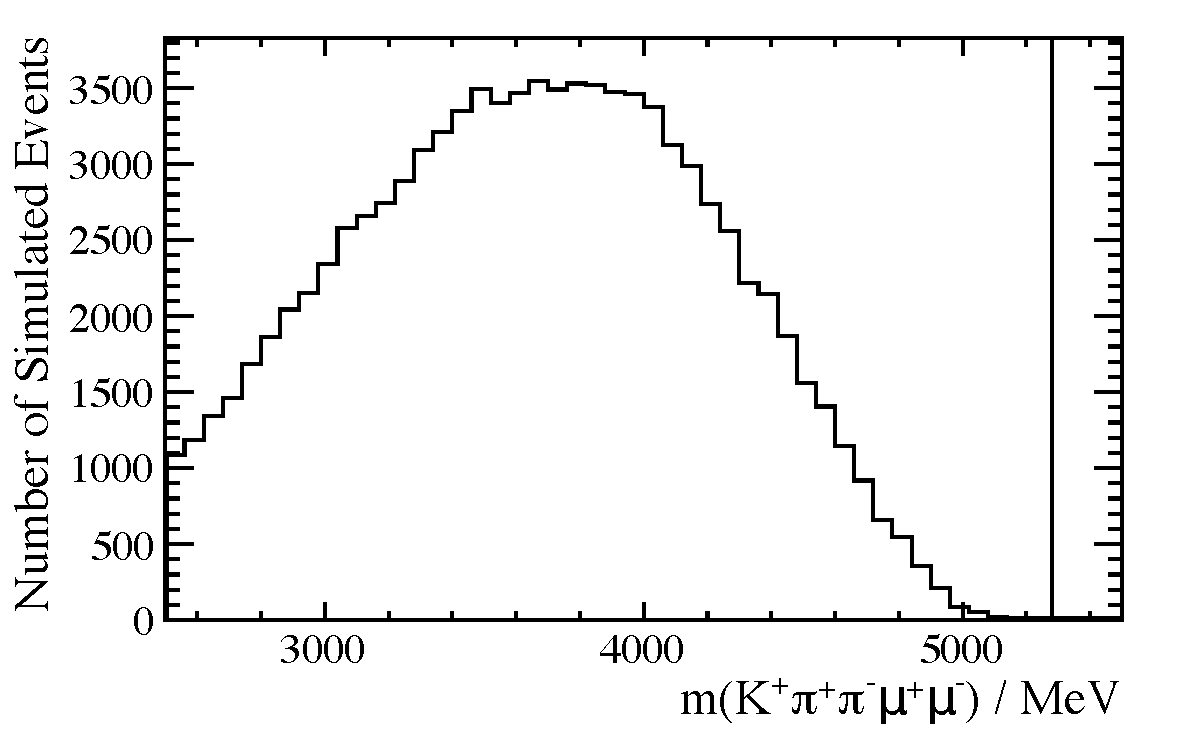
\includegraphics[width=0.48\textwidth]{hhh_cascade}
    \caption[Simulated background from cascade decays]
    {
      Background from the cascade decay $\decay{\Bp}{\Dm\pip\mup\nu_\mu}$, where
      $\decay{\Dm}{\Kp\pim\mun\bar\nu_\mu}$ does extend as high in mass as the nominal \Bp mass,
      due to lost energy from neutrinos.
      The vertical black line indicates the nominal mass of the \Bp meson.
    }
    \label{fig:hhh:cascade}
  \end{center}
\end{figure}


\subsection{Multivariate selection}
\label{sec:hhh:bdt}
Combinatorial background is suppressed using a \BDT trained using the AdaBoost
algorithm~\cite{AdaBoost}, which is described in detail in \Chap{sec:bdt:ada}, and is implemented
using the \gls{TMVA}~\cite{Hocker:2007ht}.
The signal-proxy is taken from the background subtracted sample of \btojpsikpipi candidates.
Background-like events are selected from the upper mass sideband of the signal selection in the
range $5530<\mass{\kpipimumu}<5780\mev$.
%Both signal and background samples used for \BDT training were taken from data.
%The sample of data used as the signal-proxy was from  the decay \btojpsikpipi, which had been
%\emph{sWeighted}~\cite{splot} for the purpose of removing combinatorial background from the
%training sample.
%For the background sample, selected signal mode data was taken from the upper mass sideband of the
%\Bp candidate mass, in the range $5530<\mass{\kpipimumu}<5780\mev$.
These candidates are not used for the determination of the signal yield, and at this high mass are
comprised solely of combinatorial background.

This \BDT was trained using selection of geometric and kinematic variables, the exact variables are
listed in \Tab{hhh:tab:bdtvars}.

%\begin{table}
  %\caption[\BDT training variables]
  %{
    %Input variables used to train the \BDT to distinguish between signal \btokpipimumu decays and
    %combinatorial backgrounds.
  %}
  %\label{hhh:tab:bdtvars}
  %\begin{center}
    %\begin{tabular}{lc}\\\toprule
      %Particle & Variable\\\midrule
      %\Bp & \pt\\
      %& \chisqip \\
      %& \chisqfd\\
      %& \chisqvtx\\
      %& $\theta_\mathrm{dir}$\\\littlerule
      %Tracks & \pt\\
      %& \chisqip\\
      %%\hline
      %\bottomrule
    %\end{tabular}
  %\end{center}
%\end{table}
\begin{table}
  \caption[BDT training variables]
  {
    Input variables used to train the \BDT to distinguish between signal \btokpipimumu decays and
    combinatorial backgrounds.
  }
  \label{hhh:tab:bdtvars}
  \begin{center}
    \begin{tabular}{lccccc}\\\toprule
      Particle & \multicolumn{5}{c}{Variables}\\\midrule
      \Bp & \pt
      & \chisqip
      & \chisqfd
      & \chisqvtx
      & $\theta_\mathrm{dir}$\\
      Tracks & \pt & \chisqip\\
      %\hline
      \bottomrule
    \end{tabular}
  \end{center}
\end{table}


\subsubsection{Optimisation of particle identification criteria and multivariate classifier}
\label{sssec:opt:kpipi}
The determination of the optimum cut value on the \BDT is required in conjunction with optimizing
\pid criteria on each hadron.
For the decay \btokpipimumu, a requirement that $\dllkpi(\Kp)-\dllkpi(\pip)>10$ is made, to
ensure that of the two hadrons with the same sign, the one identified as a kaon had more of
a kaon like signature than the other.
This also reduces the number of multiple candidates per event.
%Before this cut is applied $98\pc$ of events have a multiple candidates, where another candidate in
%the event is a K pi swap down to 0.
Before this cut, there is, on average, 1.32 candidates per event within $3\stdev$ of
$\mass{\Bp}^{\pdg}$, which is reduced to 1.05 candidates per event.
Then, optimisation was made in the three dimensions of \BDT, $\dllkpi(\Kp)$ and $\dllkpi(\pi^\pm)$
by maximising the figure of merit $S/\sqrt{S+B}$, where $S$ and $B$ are the expected signal and
background yields respectively.
The value of $S$ was determined by scaling the weighted sum of selected \btojpsikpipi events,
$N\big(\btojpsikpipi\big)$, according to
\begin{multline}
  S\big(\btokpipimumu\big) = \\
  \frac{
    \BF\big(\decay{\Bp}{\kone{1270}\mumu}\big)
    \BF\big(\decay{\kone{1270}}{\kpipi}\big)
  }{
    \BF\big(\decay{\Bp}{\jpsi\kpipi}\big)
    \BF\big(\decay{\jpsi}{\mumu}\big)
  }
  \cdot
  N\big(\btojpsikpipi\big).
\end{multline}
Branching fraction values used in this calculation are taken to be
$\BF\big(\decay{\kone{1270}}{\kpipi}\big) = (35.7\pm3.7)\e{-2}$,
$\BF\big(\jpsitomumu\big) = (5.93\pm0.06)\e{-2}$, and
$\BF\big(\btojpsikpipi\big) = (8.1\pm1.3)\e{-4}$~\cite{PDG2012}.
Estimation of the branching fraction of the signal decay \decay{\Bp}{\kone{1270}\mumu} is made
assuming the ratio of the branching fractions for the known decays $\decay{B}{X_s\mumu}$ to
$\decay{B}{X_s\gamma}$
is the same for $X_s\in\{\kone{1270},\Kstarent\}$.
%being the \kone{1270} or \Kstarent.
Thus,
\begin{align}
  \BF\big(\decay{\Bp}{\kone{1270}\mumu}\big)
  &=
  \BF\big(\decay{\Bp}{\kone{1270}\gamma}\big)
  \cdot\frac{
    \BF\big(\decay{\Bp}{K^*(892)^0\mumu}\big)
  }{
  \BF\big(\decay{\Bp}{K^*(892)^0\gamma}\big)
  }\nonumber\\
  &=\big(1.05\pm0.34\big)\e{-6}.
\end{align}

%This optimisation was performed using the cross-check channel \btojpsikpipi, where $S$ was defined
%as the weighted sum of events that pass a given set of cuts, and $B$ was
%where $S$ is defined as the

The value of the estimated background yield, $B$, is determined from interpolating
\btokpipimumu candidates from the mass sidebands into the regions around the mass of the \Bp meson.
Candidates falling in the low and high mass sidebands are fit to a decaying exponential, and
value of $B$ taken to be the integral of this fitted distribution within $3\stdev$ of the known \Bp
mass~\cite{PDG2012}.
Sideband regions are defined by \Bp candidates with masses between $5000\mev$ and $5750\mev$, but
more than $120\mev$ from the nominal \Bp mass.
%%$5000<\mass{\kpipimumu}<\mass{\Bp}^\pdg-120\mev$
%$\mass{\kpipimumu}\in[5000,\mass{\Bp}^\pdg-120]\mev$
%and
%%$m_{\Bp}^\pdg+120<\mass{\kpipimumu}<5750\mev$
%$\mass{\kpipimumu}\in[m_{\Bp}^\pdg+120,5750]\mev$
%respectively,


%\begin{figure}
  %\begin{center}
    %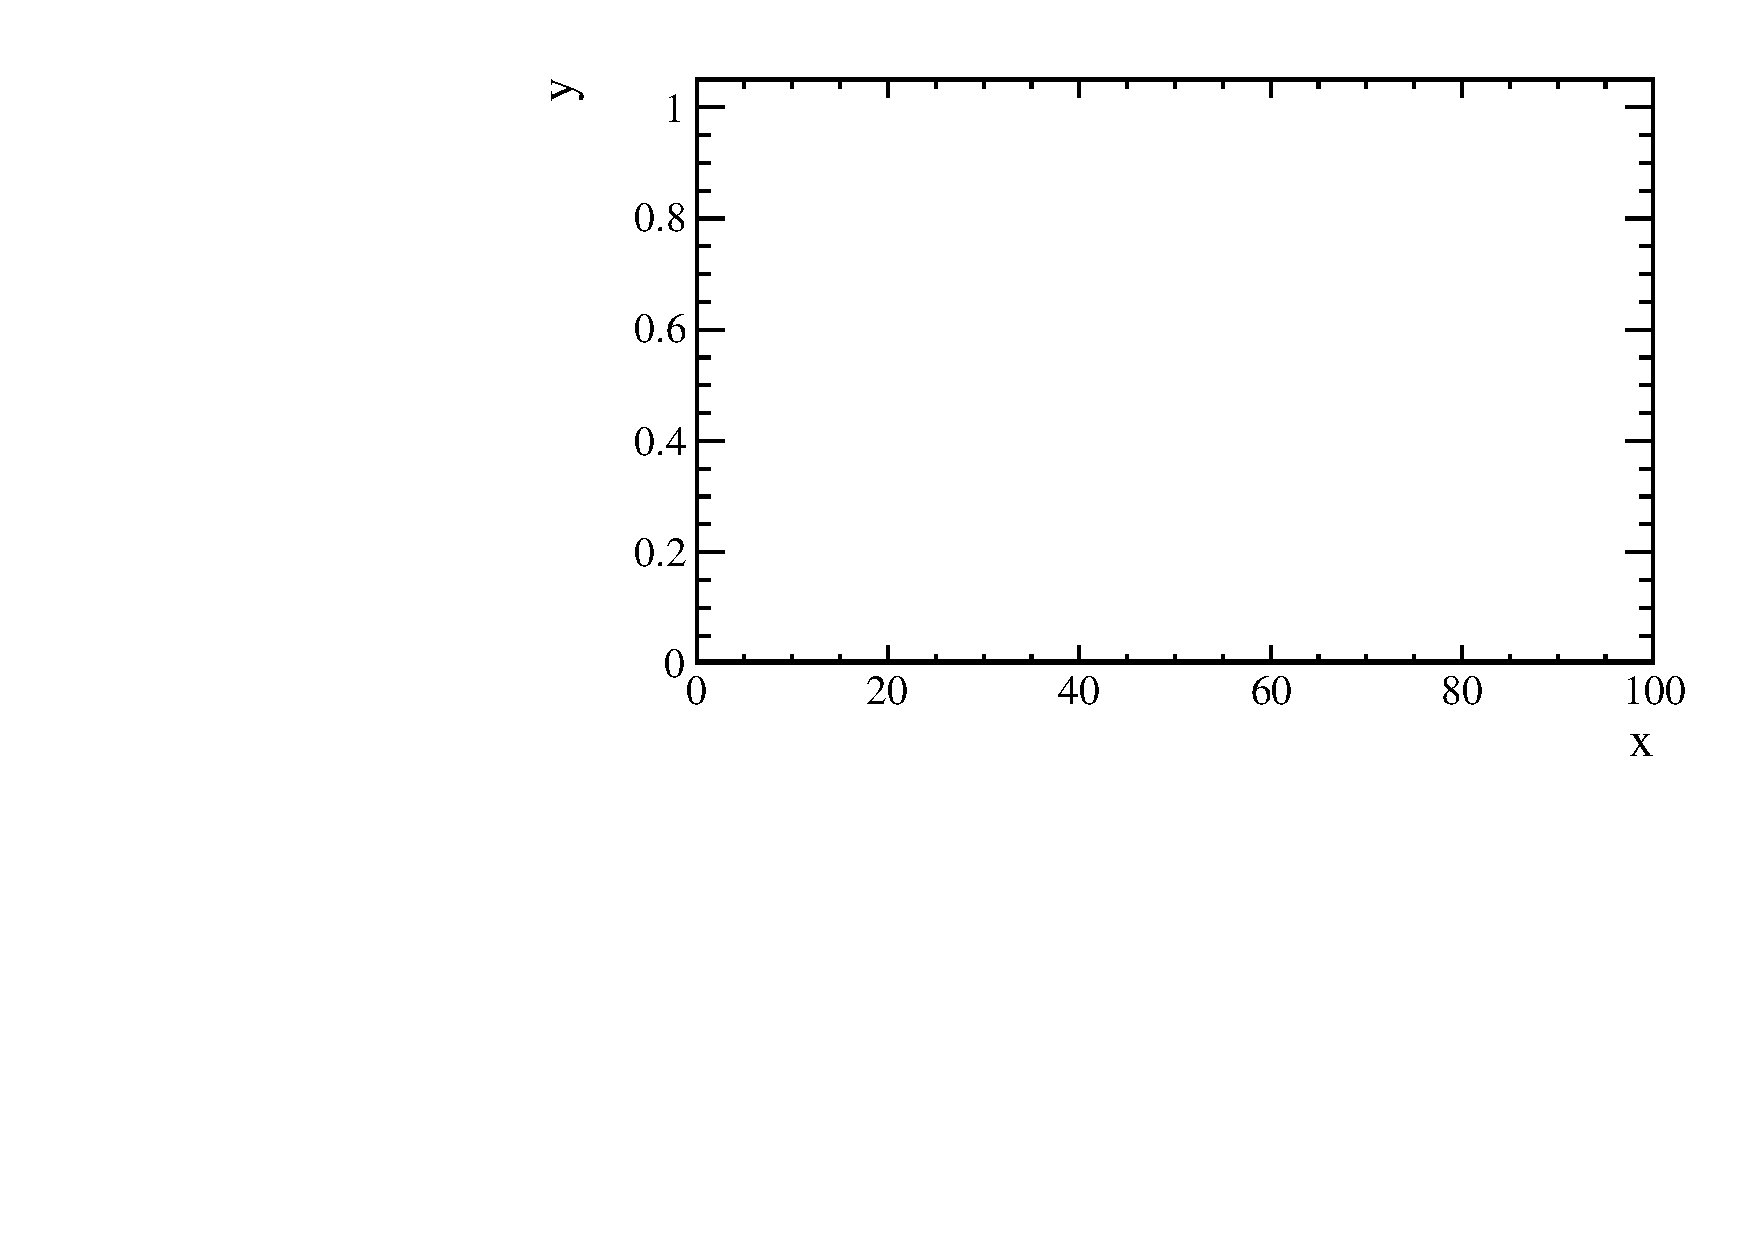
\includegraphics[width=0.48\textwidth]{blank}
    %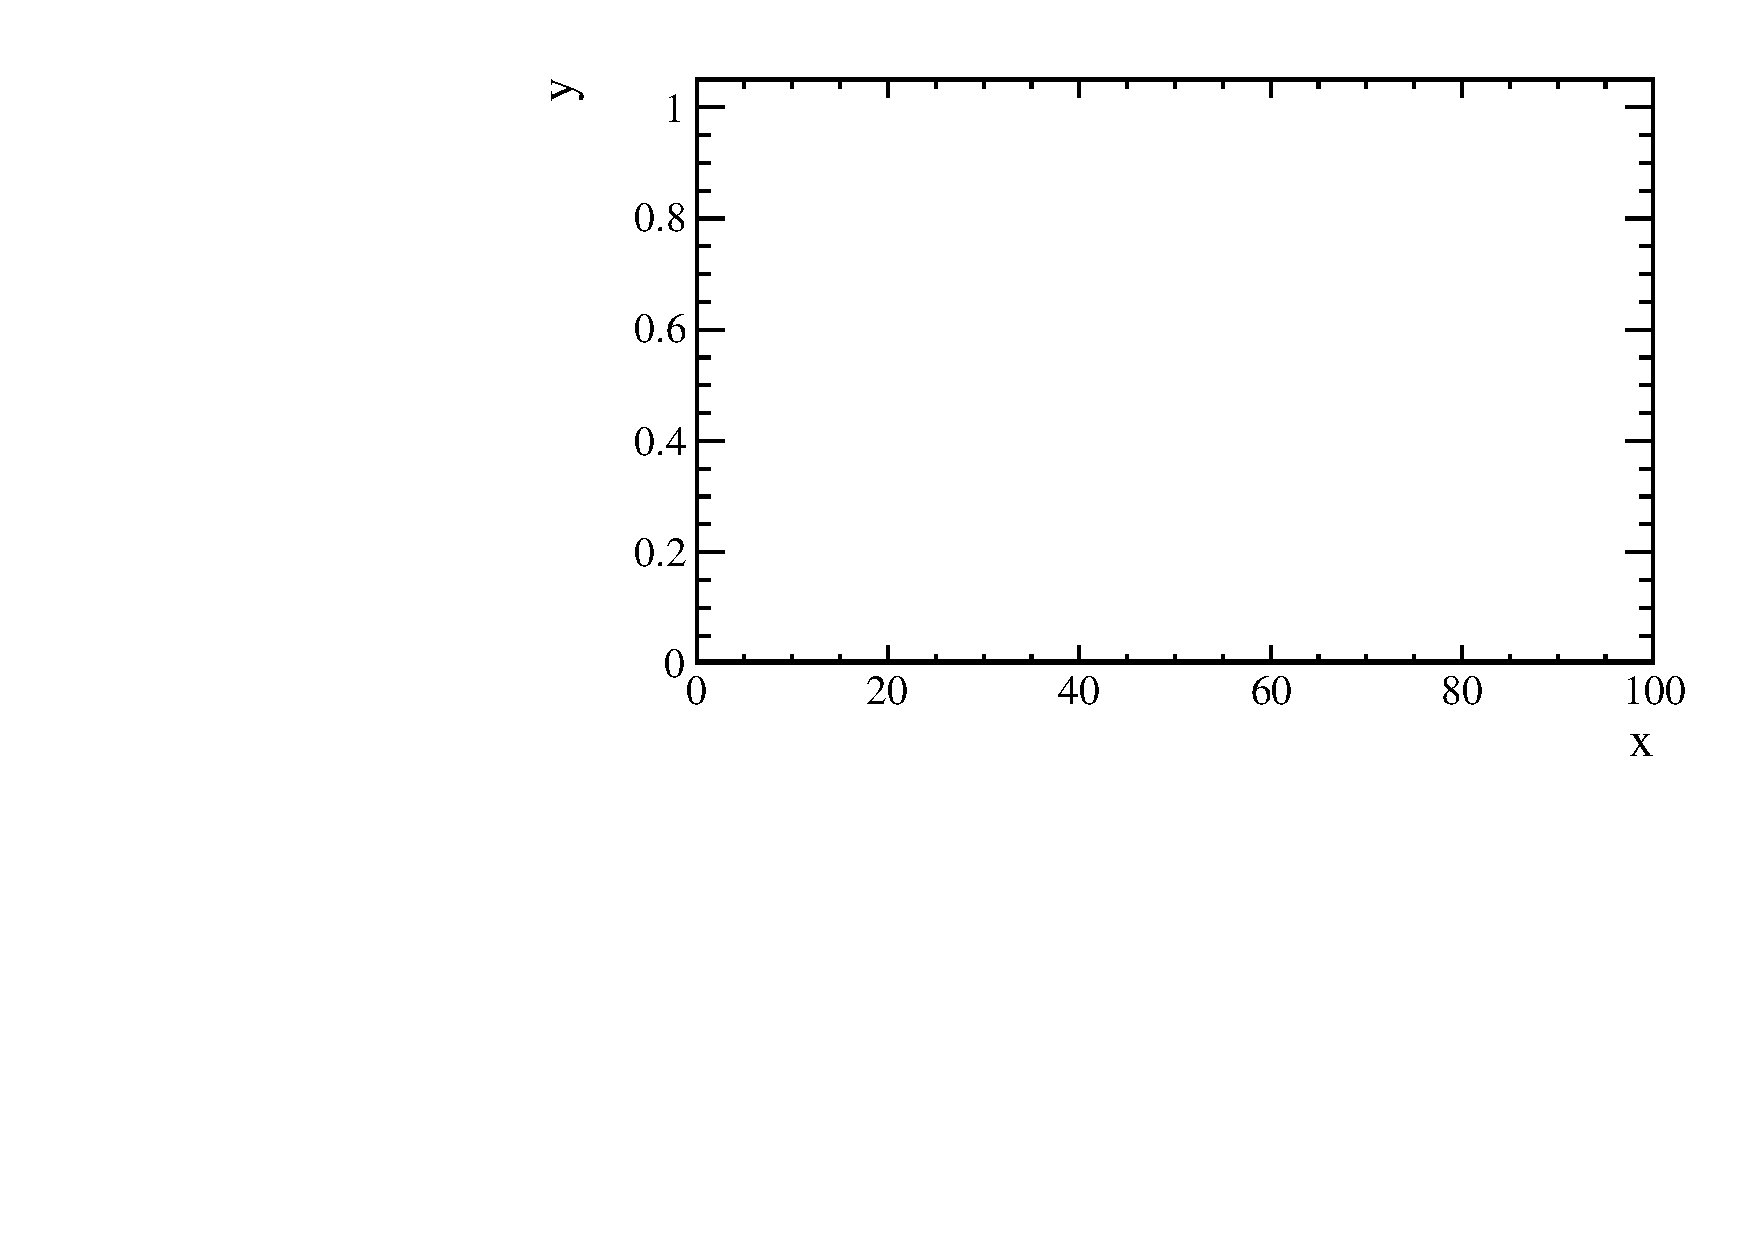
\includegraphics[width=0.48\textwidth]{blank}
    %\caption{
      %FILL IN.
    %}
    %\label{fig:kpipi:opt}
  %\end{center}
%\end{figure}


%\subsubsection[Optimisation of \btophikmumu cuts]
%{Optimisation of \tmath{\btophikmumu} cuts}

The optimisation procedure for the decay \btophikmumu employs a similar strategy as \btokpipimumu,
but only in two dimensions  (\BDT and $\dllkpi(K^\pm)$).
%This channel follows a similar procedure for optimisation as for the decay \btokpipimumu.
%Optimisation was performed in multiple dimensions (\BDT and $\dllkpi(K^\pm)$) with the chosen
%selection of cuts maximising the figure of merit $S/\sqrt{S+B}$.
The calculation of $B$ was made in the same way as described above, and the
value of $S$ was determined in a similar way, by scaling the \emph{sWeighted} sum of candidates
that passed given cuts.
So,
\begin{equation}
  S\big(\btophikmumu\big) = \\
  \frac{
    \BF\big(\decay{\Bp}{\phi\Kp\mumu}\big)
  }{
    \BF\big(\decay{\Bp}{\jpsi\phik}\big)
    \BF\big(\decay{\jpsi}{\mumu}\big)
  }
  \cdot
  N\big(\btojpsiphik\big).
\end{equation}
where $N\big(\btojpsiphik\big)$ is the weighted number of selected \btojpsiphik events.
The expected background yield is determined using an exponential fit across the signal region, as
is done for the \btokpipimumu channel.
The prediction for the branching fraction of the signal channel is taken to be
\begin{align}
  \BF\big(\decay{\Bp}{\phi\Kp\mumu}\big)
  &=
  \BF\big(\decay{\Bp}{\phi\Kp\gamma}\big)
  \cdot\frac{
    \BF\big(\decay{\Bp}{K^*(892)^0\mumu}\big)
  }{
    \BF\big(\decay{\Bp}{K^*(892)^0\gamma^{}}\big)
  }\nonumber\\
  &=\big(0.66\pm0.12\big)\e{-7}.
\end{align}
%Figure~\ref{fig:phik:opt} shows the variation of the figure-of-metrit, $S/\sqrt{S+B}$, for
%different values of the \bdt and $\dllkpi(K)$ cuts.

%\begin{figure}
  %\begin{center}
    %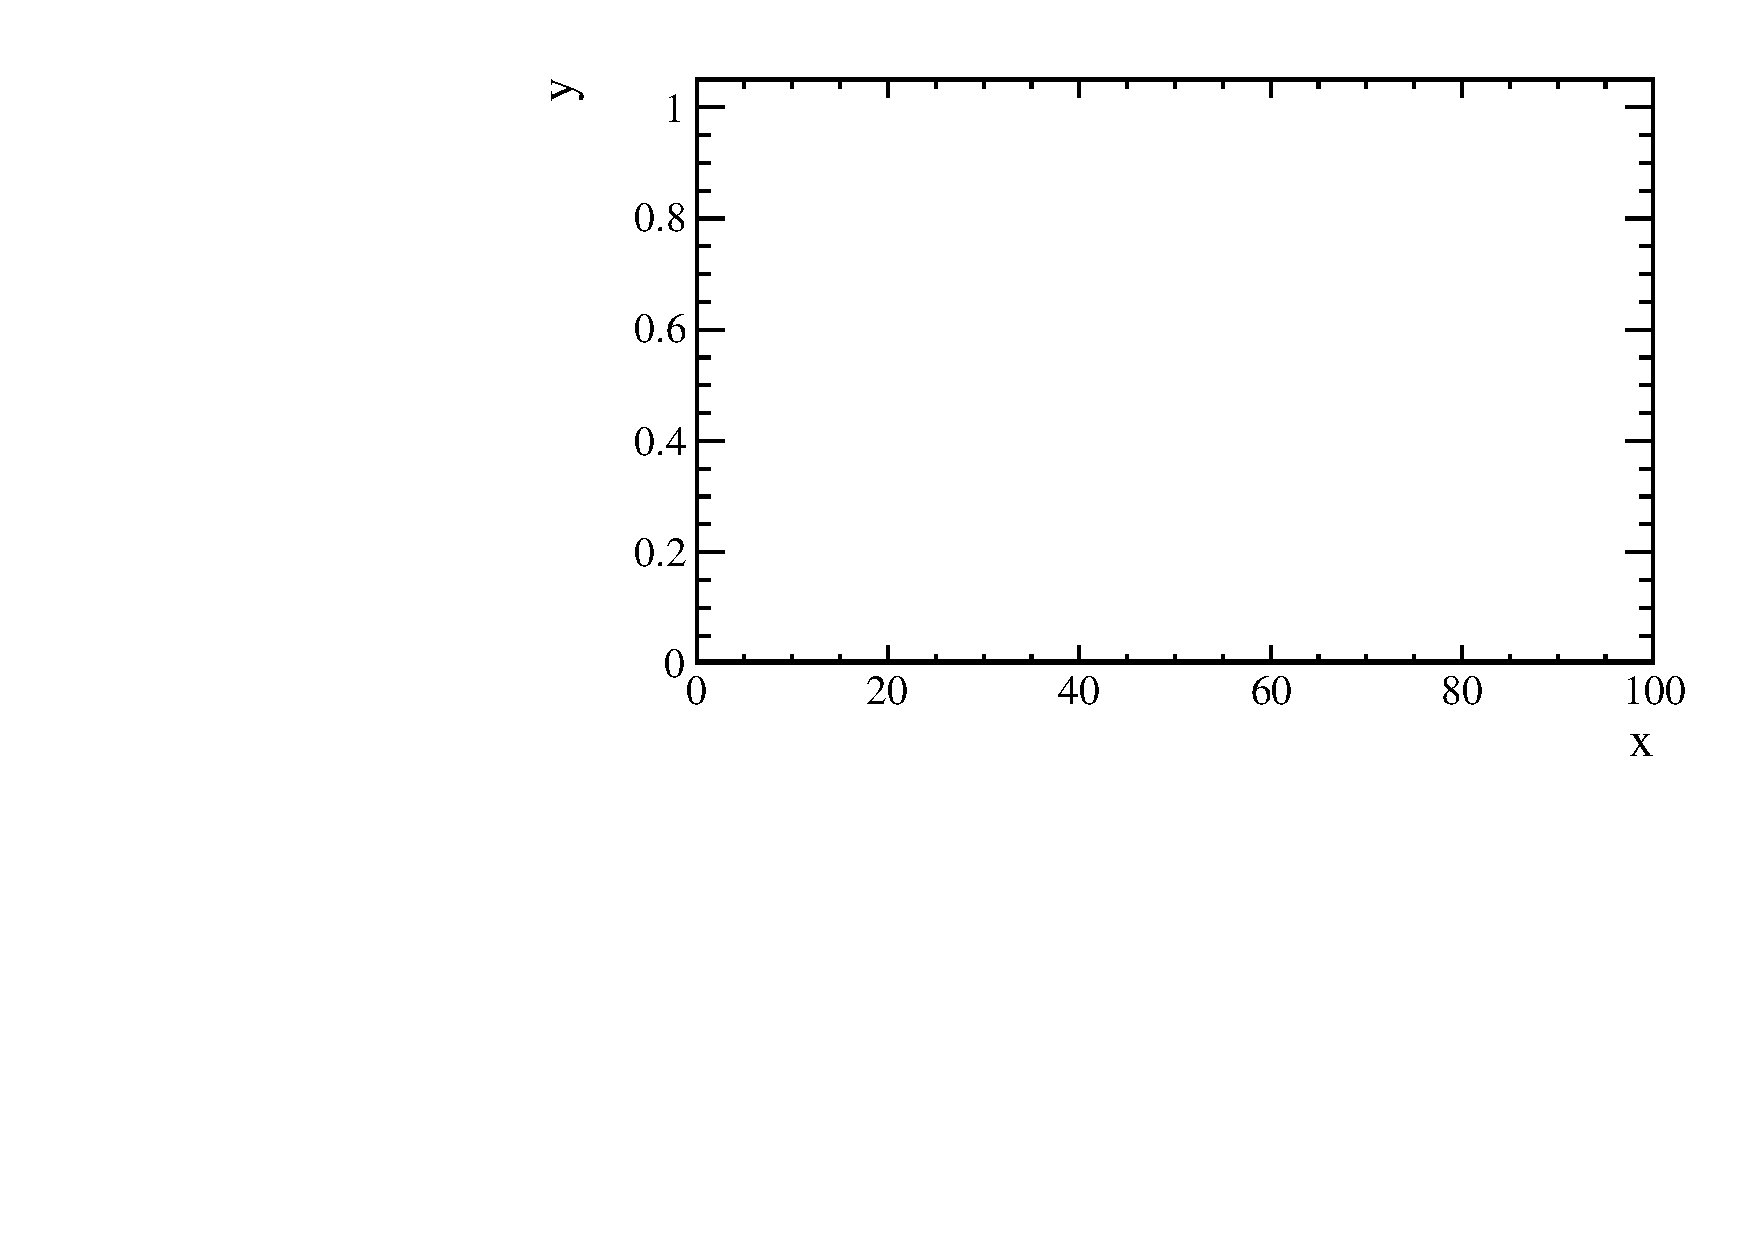
\includegraphics[width=0.48\textwidth]{blank}
    %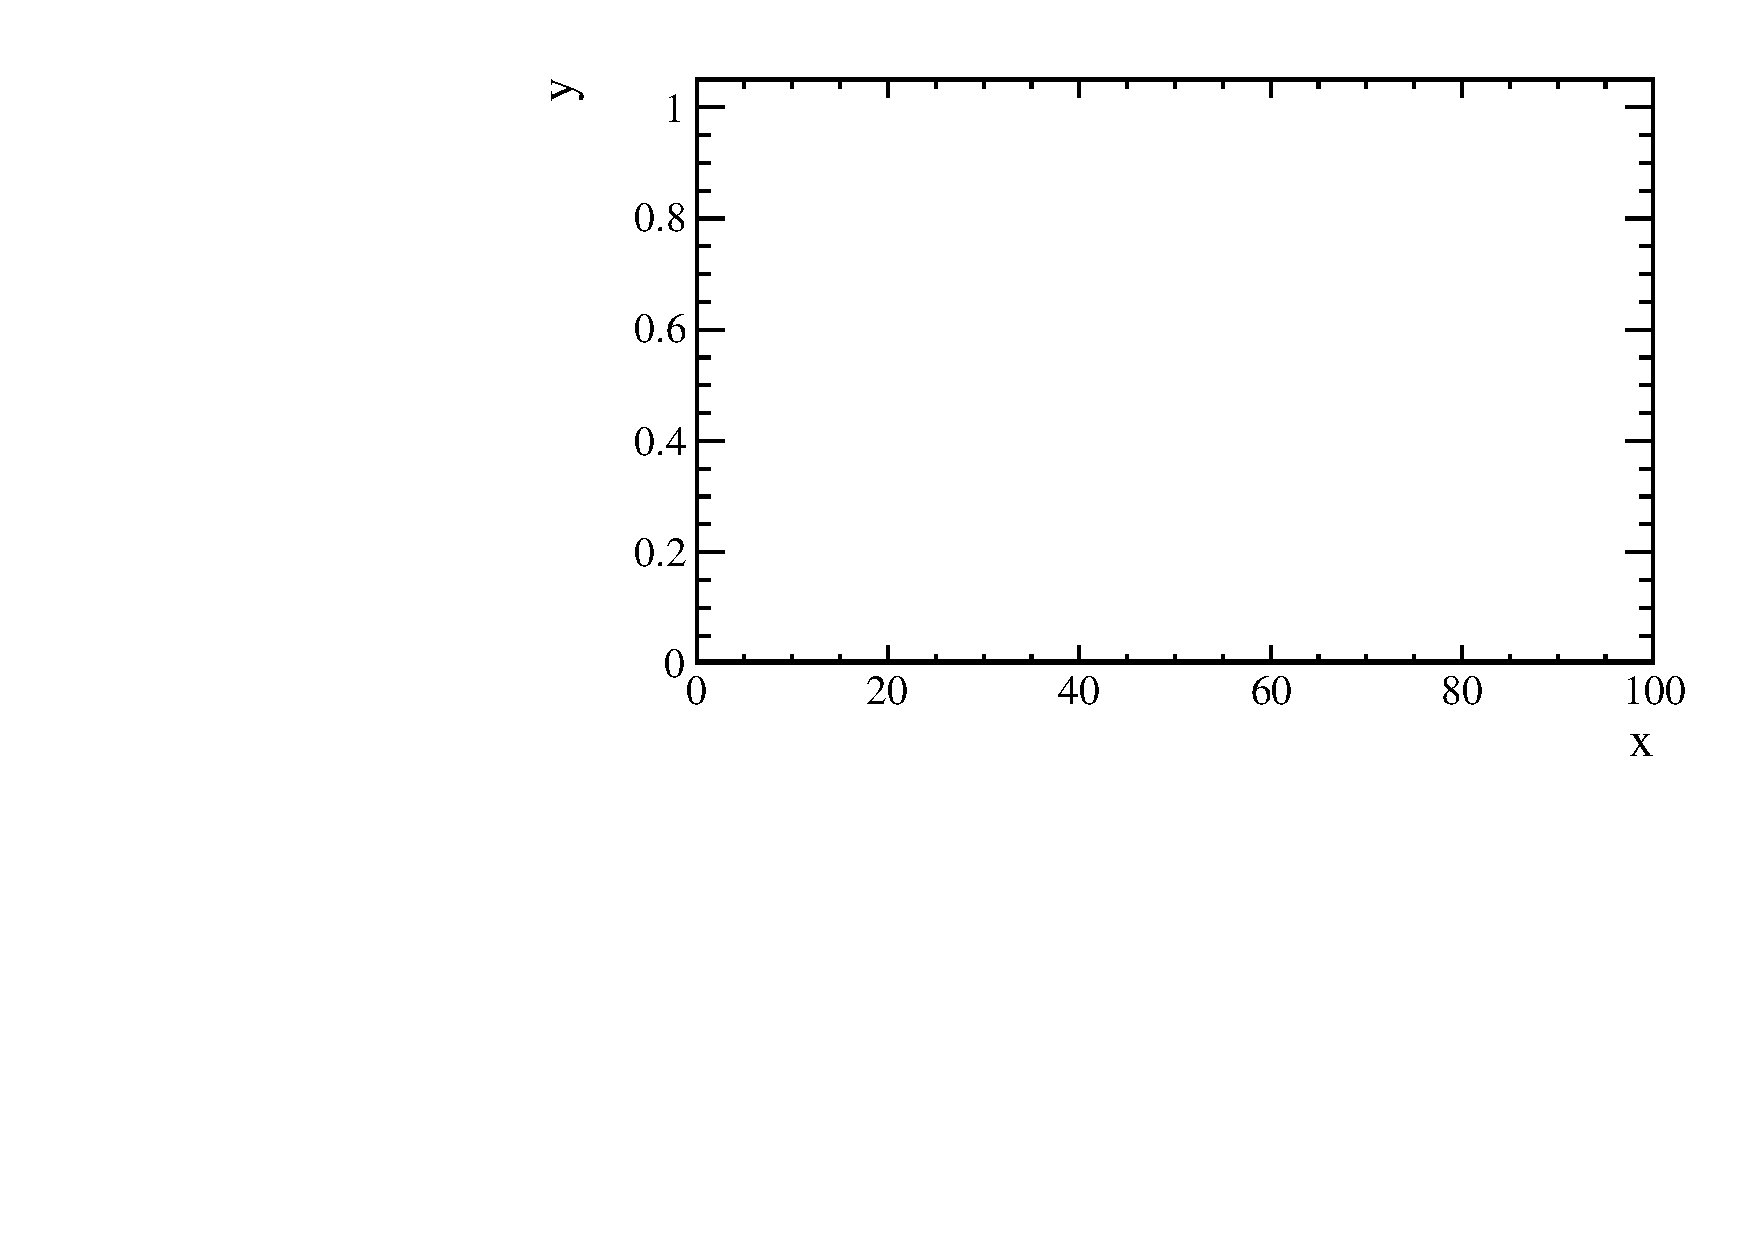
\includegraphics[width=0.48\textwidth]{blank}
    %\caption{
      %FILL IN.
    %}
    %\label{fig:phik:opt}
  %\end{center}
%\end{figure}

The maximum value of the figure of merit was found, and corresponding cut values used for the
analysis.
Exact requirements for the \pid variables were that $\dllkpi(\Kp)>3.5$, $\dllkpi(\pi^\pm)<14.5$ and
$\mathrm{BDT}>0.025$.
After the full selection multiple candidates are removed at random such that there is, at most, one
\btokpipimumu candidate per event.
For the analysis of the decay \btophikmumu, the optimisation procedure yields cut values of
$\dllkpi(K)>-3$ and $\bdt>0.05$.
The value of the \dllkpi criteria is looser for \btophikmumu than for \btokpipimumu because the
implicit \pid requirements when selecting a \phii candidate.

%\begin{table}
  %\caption[Expected yields]
  %{
    %Expected values for $S$ and $B$ for the maximum value of the figure of merit $S/\sqrt{S+B}$.
    %These are taken from the 2012 sample only.
  %}
  %\label{tab:hhh:opt}
  %\begin{center}
    %\begin{tabular}{lrrc}\toprule
      %\cellc{Decay} & \cellc{$S$} & \cellc{$B$} & \cellc{$S/\sqrt{S+B}$} \\
      %\midrule
      %\btokpipimumu & 304 & 166 & 14.0 \\
      %\btophikmumu  &  28 &   8 & \pz4.7 \\
      %\bottomrule
    %\end{tabular}
  %\end{center}
%\end{table}







%\subsection{Reweighting of variables}


%\section{Backgrounds}
%\section{Mass fits}
%\section{Efficiencies}
%\section{Systematics}
%\section{Summary}

%PID info from the RICH is used to identify final state hadrons
%PV chosen based on lowest PV of B candidates
%vertex fit \chisq must increase by more than 121 when including the B candidate daughters
%fit vertex chi2 < 6
%Backgorunds of \jpsi and \psitwos must be removed
%also their radiative tails
%main sources of peaking backgrounds come from charmonia
